\section{Evaluation}
\label{sec:eval}

We made \landslide available to students for the thread library project
during the Spring '15, Fall '15, and Spring '16 semesters of \fourten.
We introduced stateless model checking and gave a demo during a special lecture,
and required students to pass the thread library hurdle (\sect{\ref{sec:grading}}) to use \landslide.
Of 90 total two-student groups in those semesters, 47 tested their thread libraries with \landslide.

Whenever a student ran \landslide,
it recorded which options were used (test program and time limit),
a snapshot of the student's code,
and the result of the test (completed, timed out, bug found, or ctrl-C'ed).
%
We manually analyzed these snapshots to count how many bugs each group found
(not double-counting the same bug found repeatedly)
and how many of those were fixed before submission
(i.e., the students changed their code and re-ran the same test successfully).
%
We also distinguished {\em deterministic} bugs from concurrency bugs
by identifying whether \landslide needed to test multiple interleavings before finding the bug\footnote{
	For example, many students found deterministic use-after-free bugs,
	previously overlooked because the unit tests do not provide heap checking like \landslide does.
}.

\begin{table}[t]
	\begin{tabular}{r|cc|cc}
	%det bugs found	det bugs fixed	races fixed	races found
	& \multicolumn{2}{c|}{Deterministic bugs} & \multicolumn{2}{c}{Nondeterministic bugs} \\
	\# bugs	& found & fixed & found & fixed \\
	\hline
	0	& 27	& 32	& 15	& 23	\\
	1	& 6	& 5	& 7	& 11	\\
	2	& 9	& 6	& 12	& 8	\\
	3	& 2	& 1	& 7	& 2	\\
	4	& 1	& 1	& 3	& 1	\\
	5	& 2	& 2	& 2	& 1	\\
	11	& 	& 	& 1	& 1	\\
	\hline
	%Total groups
	%	& 47	& 47	& 47	& 47	\\
	Total bugs
		& 44	& 34	& 85	& 53	\\
	\end{tabular}
	\caption{Summary of how many bugs were found and/or fixed by how many groups.
	Each column counts how many groups found/fixed the number of bugs in each row;
	for instance, two groups found 5 concurrency bugs, one of which fixed all 5.}
	\label{tab:this-table-sucks-but-it's-the-best-i-got}
\end{table}

Table \ref{tab:this-table-sucks-but-it's-the-best-i-got} shows our results.
In total, \landslide found 44 deterministic bugs and 85 concurrency bugs.
\landslide found at least one concurrency bug for 32 groups (68\%),
24 of whom (51\%) were able to fix at least one,
verifying their update with a succesful re-run of the same test.

\begin{figure}[t]
	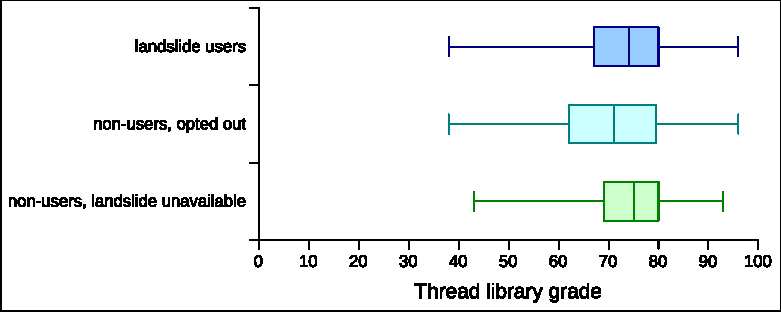
\includegraphics[width=0.48\textwidth]{p2-distribution.pdf}
	\caption{Distribution of thread library grades.}
	\label{fig:p2-distribution}
\end{figure}
We also collected the overall thread library grades to evaluate whether \landslide helps students achieve more during the project.
Figure~\ref{fig:p2-distribution} shows the distribution of these grades.
Compared to students from the same semesters who opted not to use \landslide,
those who did scored on average 3\% higher. % that's rough, buddy.
%
%However, to account for the possible bias for opting-out students being more at the bottom of the class
%on account of not enough free time to volunteer for \landslide,
However, the latter distribution is potentially biased towards struggling students
who lack enough free time to volunteer for \landslide.
To account for this, we also checked grades from prior semesters when \landslide was not available.
This distribution is indistiguishable from the experimental group,
suggesting that \landslide's benefit is largely offset by the time investment required.
%
In future work, we will streamline the user experience to help students fix as many concurrency bugs with a smaller time investment.
